% Source: graduate-coursework/Sp26/CSCE763/Course_Assignments/Exam/Midterm_Exam_solutions.tex

\documentclass[border=4pt]{standalone}
\usepackage{amsmath}
\usepackage{amssymb}
\usepackage{graphicx}
\usepackage{tikz}
\usepackage{xcolor}
\usetikzlibrary{shapes.geometric, arrows.meta, positioning, patterns, calc}

\definecolor{USC_Garnet}{HTML}{73000A}
\definecolor{USC_Sandstorm}{HTML}{FFF2E3}
\definecolor{USC_Black90}{HTML}{363636}
\definecolor{USC_Black70}{HTML}{5C5C5C}
\definecolor{USC_Black50}{HTML}{A2A2A2}
\definecolor{USC_Black10}{HTML}{ECECEC}
\definecolor{USC_Honeycomb}{HTML}{65780B}
\definecolor{USC_Atlantic}{HTML}{466A9F}
\definecolor{USC_Congaree}{HTML}{1F414D}
\definecolor{USC_Rose}{HTML}{CC2E40}

\newcommand{\problem}[1]{%
  \vspace{0.5cm}
  {\noindent\normalsize \textbf{#1}}
  \vspace{0.3cm}
}

\begin{document}
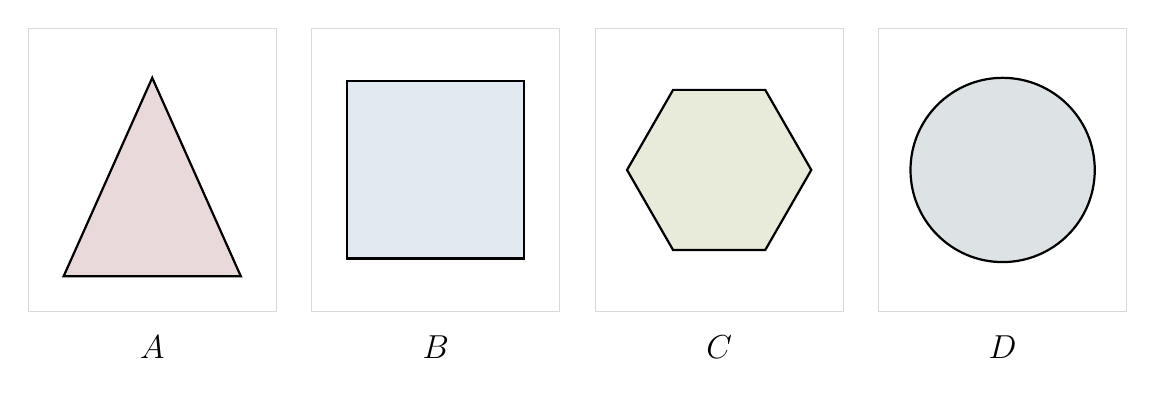
\begin{tikzpicture}[scale=0.9]

    % === Shape A (Triangle) - centered and filling box ===
    \begin{scope}[shift={(0,0)}]
        \draw[gray!30, thin] (-0.5,-0.5) rectangle (3,3.5);
        \fill[USC_Garnet!15] (0,0) -- (2.5,0) -- (1.25,2.8) -- cycle;
        \draw[thick] (0,0) -- (2.5,0) -- (1.25,2.8) -- cycle;
        \node[font=\large\bfseries] at (1.25, -1) {$A$};
    \end{scope}

    % === Shape B (Rectangle) - centered and filling box ===
    \begin{scope}[shift={(4,0)}]
        \draw[gray!30, thin] (-0.5,-0.5) rectangle (3,3.5);
        \fill[USC_Atlantic!15] (0,0.25) rectangle (2.5,2.75);
        \draw[thick] (0,0.25) rectangle (2.5,2.75);
        \node[font=\large\bfseries] at (1.25, -1) {$B$};
    \end{scope}

    % === Shape C (Hexagon) - centered and filling box ===
    \begin{scope}[shift={(8,0)}]
        \draw[gray!30, thin] (-0.5,-0.5) rectangle (3,3.5);
        % Hexagon centered at (1.25, 1.5) with radius 1.3
        \fill[USC_Honeycomb!15] (2.55,1.5) -- (1.9,2.63) -- (0.6,2.63) -- (-0.05,1.5) -- (0.6,0.37) -- (1.9,0.37) -- cycle;
        \draw[thick] (2.55,1.5) -- (1.9,2.63) -- (0.6,2.63) -- (-0.05,1.5) -- (0.6,0.37) -- (1.9,0.37) -- cycle;
        \node[font=\large\bfseries] at (1.25, -1) {$C$};
    \end{scope}

    % === Shape D (Circle) - centered and filling box ===
    \begin{scope}[shift={(12,0)}]
        \draw[gray!30, thin] (-0.5,-0.5) rectangle (3,3.5);
        \fill[USC_Congaree!15] (1.25,1.5) circle (1.3);
        \draw[thick] (1.25,1.5) circle (1.3);
        \node[font=\large\bfseries] at (1.25, -1) {$D$};
    \end{scope}

\end{tikzpicture}
\end{document}
